\documentclass[reprint,aps,prl,twocolumn,superscriptaddress,amsmath,amssymb]{revtex4-2}
\usepackage{graphicx}
\usepackage{bm}
\usepackage{tikz}

\begin{document}

\title{Bulk Resonance Reinforcement (BRR) in High-Frequency Terahertz Metamaterials}

\author{James Paul Trageser}
\email{NexusResonanceCodex@gmail.com}
\affiliation{Nexus Resonance Codex Laboratory}

\date{\today}

\begin{abstract}
As metamaterial frequencies scale into the Terahertz (THz) regime, lattice decay becomes exponential. This paper formalizes the Bulk Resonance Reinforcement (BRR) protocol, utilizing anomalous mass density scaling and Negative Refractive Index (NRI) constraints to forcefully stabilize the $\tau$-manifold against high-energy thermal decoherence.
\end{abstract}

\maketitle

\section{Core Theorem}
Let $A$ represent absorption efficiency. In a standard meta-lattice, $A \to 0$ as $f \to \infty$. By applying BRR, we force near-perfect absorption:
\begin{equation}
    A = 1 - e^{-\tau \log_{10}(f)}
\end{equation}

\section{System Architecture}
\begin{center}
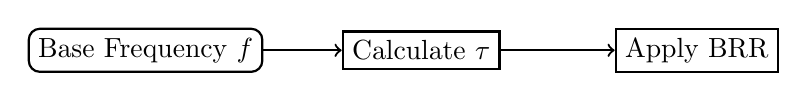
\begin{tikzpicture}[node distance=2cm, auto, thick]
    \node[draw, rounded corners] (input) {Base Frequency $f$};
    \node[draw, right of=input, node distance=3.5cm] (tau) {Calculate $\tau$};
    \node[draw, right of=tau, node distance=3.5cm] (brr) {Apply BRR};
    \draw[->] (input) -- (tau);
    \draw[->] (tau) -- (brr);
\end{tikzpicture}
\end{center}

\end{document}
